\documentclass[acmlarge]{style/acmart}

\usepackage{lipsum}
\usepackage{float}
 
%% \BibTeX command to typeset BibTeX logo in the docs
\AtBeginDocument{%
  \providecommand\BibTeX{{%
    \normalfont B\kern-0.5em{\scshape i\kern-0.25em b}\kern-0.8em\TeX}}}


 \setcopyright{acmcopyright}
 \copyrightyear{2021}
 \acmYear{2021}
 \acmDOI{}


%%
%% These commands are for a JOURNAL article.
 \acmJournal{POMACS}
 \acmVolume{1}
 \acmNumber{1}
 \acmArticle{111}
 \acmMonth{11}

\begin{document}


\title{Wireless Forensics Principles and Investigations}



\author{Evan Lomax}
\email{evn@knights.ucf.edu}
\affiliation{%
  \institution{University of Central Florida}
  \city{Orlando}
  \country{USA}
}

\author{Shenequa Hayes}
\email{shenequa.hayes07@knights.ucf.edu}
\affiliation{%
  \institution{University of Central Florida}
  \city{Orlando}
  \country{USA}
}
\author{Camilo Lozano}
\email{clozano@knights.ucf.edu}
\affiliation{%
  \institution{University of Central Florida}
  \city{Orlando}
  \country{USA}
}
\author{Shannon Padilla}
\email{jamespadilla@knights.ucf.edu}
\affiliation{%
  \institution{University of Central Florida}
  \city{Orlando}
  \country{USA}
}

\renewcommand{\shortauthors}{Lomax, et al.}

\begin{abstract}
We will discuss the current and emerging principles and investigations as it pertains to wireless digital forensics. We will look at the past, the present and future of wireless forensics. We will examine the major sub-branches, to include: 802.11 network forensics, IoT vulnerabilities, mobile forensics, available wireless security and forensics software tools. We will compare and contrast some of the major forensic tool suites as well as some emerging technologies.
\end{abstract}

%%
%% The code below is generated by the tool at http://dl.acm.org/ccs.cfm.
\begin{CCSXML}
<ccs2012>
   <concept>
       <concept_id>10003033.10003083.10003014</concept_id>
       <concept_desc>Networks~Network security</concept_desc>
       <concept_significance>500</concept_significance>
       </concept>
   <concept>
       <concept_id>10002978.10003014.10003017</concept_id>
       <concept_desc>Security and privacy~Mobile and wireless security</concept_desc>
       <concept_significance>500</concept_significance>
       </concept>
   <concept>
       <concept_id>10002978.10002979.10002983</concept_id>
       <concept_desc>Security and privacy~Cryptanalysis and other attacks</concept_desc>
       <concept_significance>300</concept_significance>
       </concept>
 </ccs2012>
\end{CCSXML}

\ccsdesc[500]{Networks~Network security}
\ccsdesc[500]{Security and privacy~Mobile and wireless security}
\ccsdesc[300]{Security and privacy~Cryptanalysis and other attacks}

%%
%% Keywords. The author(s) should pick words that accurately describe
%% the work being presented. Separate the keywords with commas.
\keywords{networks, security, IOT, 802.11}


%%
%% This command processes the author and affiliation and title
%% information and builds the first part of the formatted document.
\maketitle

\section{Introduction}
%% TODO add more introduction

In this paper we seek to provide a comprehensive overview of the current and emerging wireless security and forensic techniques used today. Wireless forensics is a vast and complex field with a rising demand for expert forensics and security professionals. By taking a deep dive in the field of 802.11 network forensics, IoT vulnerabilities, mobile forensics, and software forensics 

\section{Internet of Things}

A new growing field of devices has sprung up recently with the development and advances of the field of smart homes. These devices usually feature some sort of network connectivity either Wi-Fi or Bluetooth and are considered a form of edge computing. IoT or Internet of Things has been defined as connectable devices and sensors that allow for remote monitoring and manipulation. In a way they are considered a form of edge computing. The biggest rise in these IoT devices has been in the consumer applications smart home sector where it has really taken off in the years between 2008 and 2009 \cite{evans_iot_2011}.

The ever increasing presence of these IoT devices present a new concern as they are a prone vector for security vulnerabilities. Specially so because of the preferences for manufacturers and consumers to turn to a Wi-Fi internet solution for connecting their devices to outside. With little to no regulation, or even certifications, on how these devices can be implemented it has left a big hole in the market making it difficult to know what to trust. 
% Summary for this section might edit later
In this section we will talk about known big security exploits that have already occurred, best practices to follow, and talk about existing forensic methods that can be used to investigate these vulnerabilities.


\subsection{Background}

One of the big issues mentioned is the low level of security that is present in the IoT devices. One of the reasons they are such a threat is the current trend for these devices is to be individually connected to the internet. Initial implementations of smart home appliances relied more on a hub model where the devices were connected to a central hub. This meant that the devices were not connected to the internet and therefore had no way to communicate with the outside world except through the hub. The idea is to just expose one device to the internet and attempt to secure that one as much as possible. With the rise of cheaper micro controller boards that had built in Wi-Fi, specially the ESP8266, the standard model changed and it became more common to have each individual device connected to the main access point. One of the biggest benefits to this model is also one of its drawbacks; allowing consumers to have multiple different ecosystems. This means that there is even more potential for security attacks as each device can be from a different vendor that may or may not be secured.  

The problem becomes that in a race to the bottom of prices it has lead to corner cutting on the software side to just serve the minimum purpose without insuring any protection. We'll follow up with a couple of known intrusions that have occurred ranging from small mistakes to major security concerns. 


\subsection{Tapplock Smart Lock}

In 2018 smart device manufacturer Tapplock began selling a \$100 smart lock, mean to be a sort of gym locker lock that would allow for unlocking with a fingerprint, with a solid steel construction it also had a mobile app that would allow for unlocking the lock over Bluetooth Low Energy (BLE).
On first glance the lock boasted an 'AES 128-bit encryption', but forensic experts quickly started finding some flaws in its implementations. According to the team, they went from obtaining the lock to completely defeating its security in a mere 45 minutes! \cite{Ken_2018}

What they did was manually pair the BLE device to their computer in which they could then use a tool like Wireshark to sniff the traffic between the lock. To their surprise the lock was using HTTP API requests to control the lock over plaintext. This was the first major red flag, this means anyone able to intercept or be in the middle of the communication would be able to sniff and replicate packets to control it. 

The way they were 'securing' their requests was by using some random data attached to the request. The problem was that it was the same random data on each request, meaning that it was a symmetric key. Knowing this allows can allow for any payload for it to be sent.
Additionally another feature of the app allows for the user to share temporarily access to a guest, but as it turns out the key that you share is the same master key as the user. So even though you can set an expiration date for the guest, they essentially have access to the whole security.

The biggest revelation came from a dumping of code on the chip which revealed how the encryption key was being generated. It generates a hash based of some seed value, which turns out is just the MAC address as a string of the BLE devices, which is the only piece of data that is available to the an attacker!
This was then automated to be used in an app which would scan for nearby BLE devices and identify those that were a Tapplock device then use its MAC address to generate a key and unlock the key. Meaning that anyone with a phone in range of a Tapplock device can unlock it in less than a a couple seconds!

\subsection{Mirai Malware}


One of the most common type of internet based attacks is a Denial-of-Service (DoS) attack. This is when a malicious user or group of users is able to flood a server with requests and cause it to crash. Usually the way to prevent his is by having a firewall in place that blocks all traffic from the attacker. This is done by identifying some sort of pattern in the traffic and blocking it. An advanced form of this attack is a Distributed DoS (DDoS), which consists of a coordinated attacked by many with varying ranging IPs that would be much harder to identify and block. 

In 2016 a botnet malware started to randomly appear. A large amount of CCTV, routers and other IoT devices were being compromised by this malware. It was specially hard to detect as the IoT devices remained mostly fine except for every now and them some sluggishness every and increased bandwith. What was interesting is that this malware is that it is not complex in its nature. What it does once a device is infected is randomly scan for IPs and attempt to ping them on certain known ports. The developer compiled a list of known manufacturers default ports, usernames and passwords. Each node then just attempts pinging until it finds an open device, then its IP is uploaded to a controller that then contacts the other nodes to try to authenticate on the known device until eventually some are compromised by their default passwords. 

Once inside on a compromised device, the malware installs itself on the new device and continues to propagate. This allowed the malware to scale massively. This was then used to DDoS a bunch of websites, including a OVH (one of France's largest hosting companies), Dyn (a DNS provider), and even a cyber security journalist. At its peak there was a recorded bandwidth hitting 1 Tbit/s!\cite{Hertzberg_Mirai_2016}

Most interestingly the was that the source code of the malware was eventually leaked and the creator was identified! Apparently the author had a IT security company that offered protection against DDoS. In a way they were running a protection racket, initially starting with Minecraft servers.

This attack revealed how major manufacturers were using default credentials and allowing easy exploitable security issues. Since the code has been open sourced others have taken to fork it and adapt the same concept to different devices.

\subsection{Best Practices}

While there is many attack vulnerabilities by just using these IOT products it does not mean that you are always sacrificing security and privacy for using these devices, there a couple best practices that are recommended to take in order to prevent some of the most common attacks. One of the most recommended things that you can do is having a separate network for any IOT device. This can take many different forms, the easiest being is enabling the guest network option that is available on some routers. The router can create a secondary network for guests, but in this case you create it (and use WPA2/WPA3 to secure the network) and only use it to hook up those devices. The idea behind this being that even if there were some malicious software running on the IOT those devices could not connect to the other devices and sniff data off the network because your other phones and computer devices would be on a different network they can not access. Another way to implement this is setting up a different subnetwork and have a MAC filtering to do this but it is a more complicated approach. 

When it comes to home appliances and automation the best most secure approach is to have your own self hosted solution such as running Home Assistant and having that be the main interface for your other devices. Home Assistant supports a multitude of different IOT devices, but the best in these case are those that are those IOT devices that support ZWave, or ZigBee as their main networking interface as the device itself is not connecting to your home network rather a hub which controls what data goes in and out. There are now more common off the shelf appliances that can serve as the hub such as Samsung SmartThings and certain Alexa devices, but nothing could be more secure than hosting your own.


\section{802.11 Vulnerabilities}


\subsection{Background}

WiFi was derived from the 1971 ALOAHnet that connected the Hawaiian islands with a UHF wireless packet network. However, it was not until 1997 that the 802.11 standard was released. Numerous amendments and revisions aside, the basic foundation of WiFi has not changed drastically. Most advances center around security protocols and speed or efficiency enhancements. Early security protocols included Wired Equivalent Privacy (WEP) and WiFi Protected Access (WPA). Many vulnerabilities were discovered in these protocols and were quickly replaced with WiFi Protected Access version 2 (WPA-2). WPA-2 is the current standard, but will be soon replaced with WiFi Protected Access version 3 (WPA-3) \cite{berg2011ieee}.


\subsection{WPA2 Vulnerabilities}


In 2017, Mathy Vanhoef of imec-DistriNet discovered a serious weakness in WPA2. He determined that attackers could use key reinstallation attacks (KRACKs) which would effectively decrypt transmitted data. This vulnerability was found in the WPA2 protocol itself and any implementation of WPA2 is likely to be vulnerable. This is thought to be the first exploit of the protocol itself. Previous attacks exploited flaws in the WiFi Protected Setup, drivers, random number generators, predictable pre-shared keys and insecure enterprise authentication. 
The attack centers around the 4-way handshake utilized by the WPA2 protocols. Connection to a WiFi network starts with an authentication and association to an access point. During this stage, it is considered an Open System authentication, as it is merely an introduction.  As the handshake continues, a Pairwise Transient Key (PTK) is created. The PTK is generated from the Pairwise Master Key (PMK), Authenticator Nonce (ANonce), Supplicant Nonce (SNonce), and the MAC addresses of the requesting machine and access point. Upon generation, the PTK split into a Key Confirmation Key (KCK), Key Encryption Key (KEK), and a Temporal Key (TK). KCK and KEK are used to protect the handshake messages, whilst the TK protects normal data frames \cite{vanhoef2017key}. See Figure \ref{fig:4way}.

\begin{figure}[H]
  \centering
  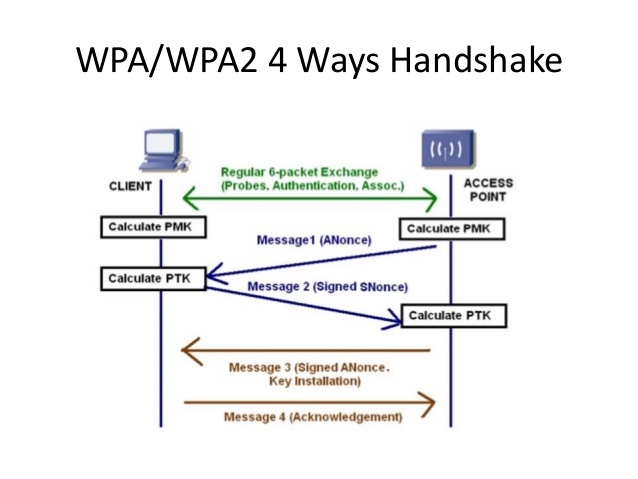
\includegraphics[width=0.5\linewidth]{imgs/wpa-4way.jpg}
  \caption{4-way Handshake \cite{t_2021}}
  \label{fig:4way}
\end{figure}

The attack occurs during message #3 of the 4-message handshake. The access point will retransmit message #3 if does not get a response. This retransmission causes a reset in the incremental packet number and the receive replay counter. A man in the middle attack can trap message #3 and force this reset and a previously used encryption key used. This also causes a reuse of previous keystream to encrypt packet data. If the packets have known content, it become quite easy to derive the previously used keystream. Obtaining the keystream allows for the attacker to decrypt messages containing the same nonce.
This vulnerability could allow attackers to obtain sensitive data. In addition, they could also inject ransomware or malware into the stream of data. An attacker could also hijack a website and provide an alternate destination in order to collect sensitive information. Interestingly enough, the attack cannot obtain the encryption keys or WiFi password.

\subsection{WPA3 Vulnerabilities}

Beginning in July 1, 2020, WPA3 became the new standard and all devices that carry the WiFi certification must be in compliance. However, once again, Mathy Vanhoef has discovered a potential new attack to the WiFi technology. He has dubbed this security vulnerability as the fragmentation and aggregation attacks (FragAttacks). This attack does require that the attacker be in range of the network, so exposure is limited. However, three of the new vulnerabilities are design flaws in the WiFi standard which exposes most devices to attack. The shining light is that most of these exploits require user interaction or uncommon network settings, so in practice these vulnerabilities are limited in scope. The biggest issue lies in the programming mistakes found in WiFi products, which makes them easy to exploit. These exploits allow for the theft of sensitive data as well as allow access to devices connected to your network \cite{vanhoef2021fragment}.

Many access points and WiFi devices accept fragmented frames as a normal course of function. While this may be common, reassembly of the frames has little to know validation. Attackers can submit fragments which have different keys which goes unnoticed during reassembly. In addition, aggregated frames include a flag to indicate aggregation, but it is not validated.



\section{Mobile Forensics}
\subsection{Introduction to Mobile Forensics}
Mobile device forensics is a subcategory of digital forensics.  It involves the recovery of digital evidence or data from any mobile device.  These mobile devices include mobile phones, smart phones, tablets, personal digital assistants (PDAs), and Global Positioning Systems (GPS).  Another type of mobile device is wearable technology, for example an Apple watch or Fitbit fitness tracker.  These types of mobile devices can store several types of private information.  This information consists of call history, contact list, incoming and outgoing text messages, pictures, videos, audio files and voicemail messages. With the usage of smart phones, the data set also comprises internet browsing history, previous Wi-Fi connections, calendars, analytical information, geolocation data, and documents.  Some people have been known to save notes with account user credentials, passwords, and passcodes in their mobile devices as well.  All this information could be useful in an investigation.  Given the wide variety of mobile devices, there are different ways each device version must be handled.  The differentiation of the data on the device depends on the cell phone generation, the device brand, and the version of the specific model.  As a part of digital forensics investigations, there are specific tools that should be used to ensure the integrity of the mobile devices during transport from one place to the next.  Additionally, there are various data collecting techniques used for data analysis and preservation.

\subsection{Progression of the Cellular Networks}
Cellular networks and technologies have changed massively since their arrival in the late 1970s.  The first-generation mobile networks started in Japan in 1979 before other countries like the US and United Kingdom.  This technology was known as the advanced mobile phone system (AMPS).  The AMPS used frequency division multiple modulation and only had a capacity of 30 kilohertz and 2.4 kbps of speed.  The 1g network only allowed voice calls and had limited protection against hackers.  The second-generation network started around 1991.  This system was based on digital signals from the global system for mobile communications (GSM).  The 2g network offered bandwidths of 30 kHz to 200 kHz.  The users could also send SMS/MMS messages up to 64 kb.  Soon after, 2.5g was established and enabled data rates up to 144 kbps.  These rates allowed for browsing the web and sending   and receiving email messages. In the year 2000, the third-generation network was introduced in Europe as UMTS and CDMA in the US.  The introduction of 3G became more about social connections and supported higher speeds.  The 3G upgrade also enabled video calls, sharing files, watching television, and more surfing the internet and now for playing online games.  The fourth-generation network era brought about the usage of smartphones and other handheld devices.  These devices have speeds from 10 Mbps and 1 Gbps.  Fourth generation was the first cellular network generation to use long term evolution (LTE), which offers users better voice quality, less buffering time, instant messaging and social media, faster downloads, and quality streaming.    The 4G cellular network is also the first IP based mobile network with the technology to accommodate the quality of service and requirements including broadband access, multimedia messaging services (MMS), video chat, mobile TV, HDTV content, and digital video broadcasting.  As the 4g network tries to keep up with the demand of augmented reality and development of autonomous vehicles, the 5g revolution has begun.  The 5th generation network is being created to enhance the growing rate of new mobile applications and standards.  The output of 5G devices is 1000 times faster than 4G at 10 Gbps and will support the number of IoT (internet of things) sensors and devices.  

\subsection{Mobile Phone Types}
When discussing cell phone brands, we all have our own personal preferences.  The reason why we like specific brands could be user friendliness, customization capabilities, security resources, the price or just the look of the device.  In mobile device forensics you must be knowledgeable of data extraction from all mobile phone brands.  There are two major mobile phone manufacturers that everyone uses, which are Apple and Samsung.  These manufacturers also develop tablets and other personal devices that use similar operating systems to the mobile phones.  Because the operating systems are similar, the same tools can be used for testing.  To begin analysis, you must identify the hardware type and the firmware that has been installed.  For the Apple iPhone, this information has been impressed onto the back of the devices shell.  This information could also be access by navigating to the phone menu settings/general/about/version.   Once you have this information, you would use software, acquired from a reputable site for Apple device evaluation, loaded on a removable drive or disc to communicate with the device.  This software will have a list of commands to use for data extraction.  When searching for the software information on an Android device, you would go to menu Settings/About Phone/Software Information.  For Android device analysis, you would download Android software development kit.  Hardware and software analysis vary for mobile devices because of the numerous brands and versions.  For this reason, there is not a universal solution for analysis nor acquisition of all cell phones and other mobile devices.

\subsection{Device Preservation and Data Collecting Techniques}
Data collecting and preservation for mobile device forensics is getting more complicated as the devices advance.  Mobile devices are used for both personal and professional purposes, so the data contained reflects that.  To recover the digital evidence and other relevant data, you must follow the guidelines for preservation and examination.  All the methods and techniques must be forensically sound, meaning all actions and processes used must respect international guidelines and avoid the alteration of the original devices.  For mobile device forensics, digital forensics in general as well, evidence should always be preserved in process in a manner that allows it to be used in a court of law.  When moving mobile devices from the scene, there are two things to consider: lock activation and network/cellular connection.  Preventing network connection is important to ensure that the mobile device is not changed remotely.  The mobile device can be isolated by placing the device on airplane mode to disable Wi-Fi and hotspots.  It is also important to make sure the device has a full charge to avoid shutdown.  During storage and transportation, Faraday bags are a great tool to use.  A simple Faraday bag will isolate the device from receiving radio signals while keeping the device charged with an emergency battery.  All original cords and chargers should be removed from the scene and secluded away from the device.  Faraday cases are made from silver, copper, or nickel.  They have RoHS (Restriction of Hazardous Substances) double layer conductors, which are best for blocking EMF (electromagnetic fields) signals.  Another tool that could be used for isolation during transportation is a jammer.  A jammer sends radio waves with the same frequency as mobile phones, which causes interference between communications and paralyzes every phone in the range of the jammer.  In some countries jammers are illegal and are only allowed to be used by law enforcement.  There are many data collecting techniques.  Your plan of execution as a digital forensics professional, must include an outline of actions taken in sequence.  This is necessary because the process may have to be duplicated at another time.  Mobile forensics data collecting methods can be non-invasive and invasive.  As a good rule of thumb, always start with non-invasive techniques because “they tend to endanger the device is integrity to a lesser degree” (Kostadinov, 2019).  Types of noninvasive mobile forensics data extraction methods include manual extraction, logical extraction, hex dump, and JTAG.  When arriving at the crime scene some devices may already be unlocked.  If this is the case, then manual extraction is possible.  Manual extraction is when you browse through the mobile device’s data by using the touch screen or keypad.  Ideally during manual extraction, you would document and take photos of the device while you're browsing.  Logical extraction involves connecting the mobile device to a forensically sound workstation.  The connection is established by using USB cords, Bluetooth, or RJ-45 cables.  Command requests for data retrieval from the computer to the mobile device.  With this method, data could be added to the mobile device altering the integrity.  The hexdump process is performed when the mobile device is connected to a forensically sound workstation, then using a bootloader a set of instructions will be delivered to dump the memory from the phone onto the computer.  A downside of this method is that the format of this data will be binary.  However, deleted data can be recovered with this process.  When using the JTAG method, you connect to test access ports on the mobile device, then send commands to the processor to transfer the raw data stored on memory chips.  This technique is a favorite among digital forensics professionals because you can gain access to the mobile devices memory without risking the integrity of the device.  However, this procedure takes more time and requires an extensive knowledge of JTAG for different models of mobile devices as well as an approach to arrange the binary data retrieved.  Invasive mobile forensics data extraction methods are more time consuming and more complex.  These methods are ideal when a device has been severely damaged and is no longer functional.  In this case the flash memory chips from the device will have to be removed and a forensic image taken.  The types of invasive mobile forensics data collection techniques are chip off and micro read.  The chip off method refers to the data being retrieved directly from the mobile device’s memory chip.  First the chip would be detached from the mobile device and inserted into a chip reader or, if applicable, a second phone could be used to read the data from the chip.  Cloning the chip from the mobile device may also be necessary if it is not severely damaged. The chip off technique is difficult because there are different types of memory chips used in mobile manufacturing.  There is a lot of training that an examiner must complete in order to apply this method in any investigation.  Additionally, special hardware may be required to work with the memory chips from the devices.  The other invasive technique used for data extraction on mobile devices is micro read.  The micro read method requires the usage of electron microscope to analyze data seen physically on the memory chip.  This technique requires the maximum level proficiency from the mobile forensic expert.  

\subsection{Last Thoughts for Mobile Forensics}
	Mobile forensics is the branch of digital forensics investigations that involves data retrieval from mobile devices.  The examining of these various devices depends on the type of device as well as the company who produces it.  Knowing how to analyze the mobile device is also determined by the version and model.  The condition of the mobile device at the scene will depict which data collecting technique will be best to perform.  As the mobile device industry evolves, future data collection techniques will have to be created in order to keep up with the times.  Currently automobile manufacturers are racing to develop autonomous vehicles, so where in the forensic spectrum will those fall?

\section{802.11 and Mobile Forensic Tools}

802.11 or “WiFi” has become normal not only in the workplace but also at home. Because of the common use of this technology, it has become necessary to develop tools and techniques in order to conduct forensic investigations on WiFi networks. These tools can simply be used to monitor traffic to find out why a network may be running slower than normal or they can be utilized for in-depth investigations because of an attack. There are also several tools and techniques for attackers or hackers to utilize in order to inject malicious packets, intercept packets, and crack network passwords in order to gain unauthorized access to a wireless network. 
There are several avenues for an examiner to conduct a forensic investigation into a wireless network. The first is examining frames on the network and capturing network traffic or packets utilizing tools and hardware. This will allow the examiner to inspect communications between stations. Packets can also contain clear-text data if unencrypted or if the encryption key is known. Most WiFi networks will typically operate in either 2.4GHz or 5 GHz radio frequency ranges. WiFi ranges are broken down into smaller bands called channels. 2.4GHz band will have 11 channels and 5GHz band will have 45 different channels. 
Wireless Access Points (WAP) can also contain fruitful information for a forensic examiner. WAPs can contain stored logs which will illuminate connections whether they were successful or not. The logs could also contain data about the attempted or successful connection such as IP and MAC addresses as well as timestamps. 
%Below is a screenshot example of a wireless log from a WAP:

\begin{figure}[H]
 \centering
  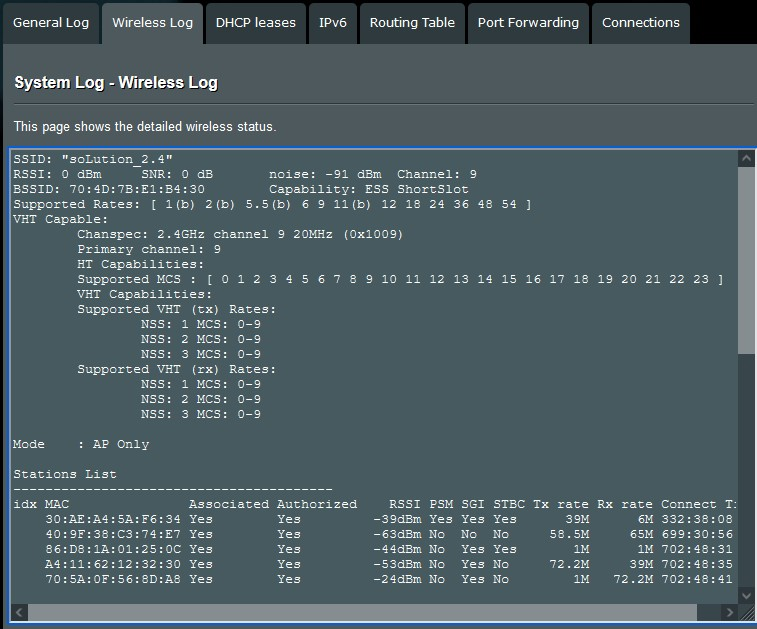
\includegraphics[width=0.5\linewidth]{imgs/waplog.jpg}
  \caption{Screenshot of a wireless log from a WAP}
  \label{fig:waplog}
\end{figure}

This particular log shows real-time connections which can be volatile. Forensic examiners can use real-time logs to determine if an unauthorized client is connected but historic logs can obviously be extremely useful as well. 

\subsection{Wireshark}

In order for an examiner to capture network traffic, an 802.11 wireless card with “monitor mode” capability is required. Wireshark is a useful tool and probably the most used by forensic examiners for monitoring network traffic live and examining historic pcap files. Wireshark allows the examiner to analyze traffic and filter exactly what they are looking for. 
%Below is a screen shot of a live capture using Wireshark:

%\begin{figure}[H]
%  \centering
%  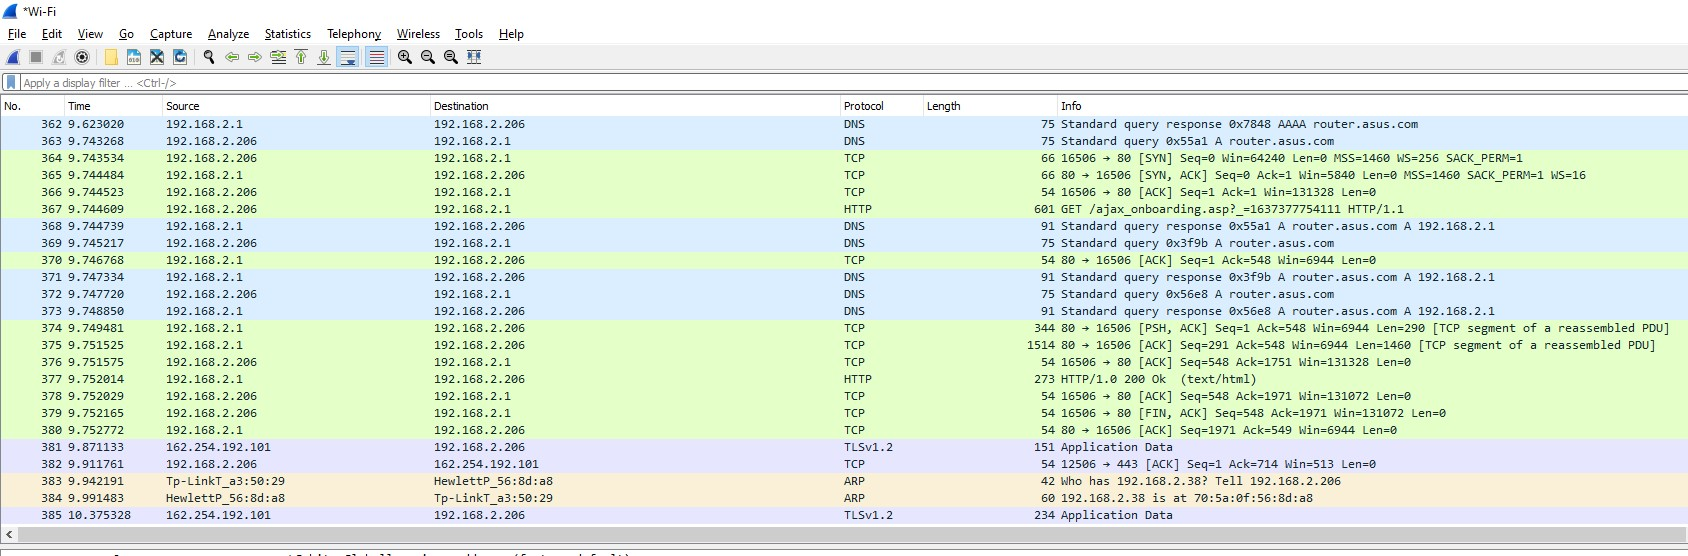
\includegraphics[width=0.5\linewidth]{imgs/wireshark.jpg}
%  \caption{Screenshot of Wireshark log}
%  \label{fig:wireshark}
%\end{figure}

Wireshark displays tons of data on each packet to include packet number of the capture, source IPs, destination IPs, protocols, frame information, mac addresses and packet data. 

\subsection{Snort}

Snort is another tool that can be utilized by an examiner to analyze network traffic. Snort is different from Wireshark in the fact that it can also be used as an Intrusion Protection System. Snort is a type of tool that an enterprise client would likely use such as a network administrator for a company. Snort can alert users of malicious packets set by rules and also log packets for historic analysis. 
%Below is a screenshot of the Snort interface:

%\begin{figure}[H]
%  \centering
%  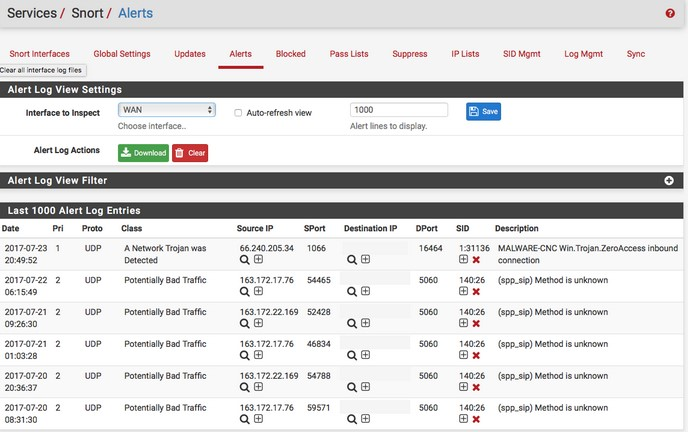
\includegraphics[width=0.5\linewidth]{imgs/snort.jpg}
%  \caption{Screenshot of Snort interface}
%  \label{fig:snort}
%\end{figure}

\subsection{Engage}

Several tools that examiners utilize in 802.11 forensics can also be used by attackers for malicious purposes. One such tool is the Engage Packet Builder tool. The Engage Packet Builder tool allows the user to create/inject packets and most notable allows the user to be able to spoof their IP address to become anonymous. This tool can be used for DOS type attacks. 
%Below is a screenshot from the Engage Packet Builder tool’s interface:

%\begin{figure}[H]
%  \centering
%  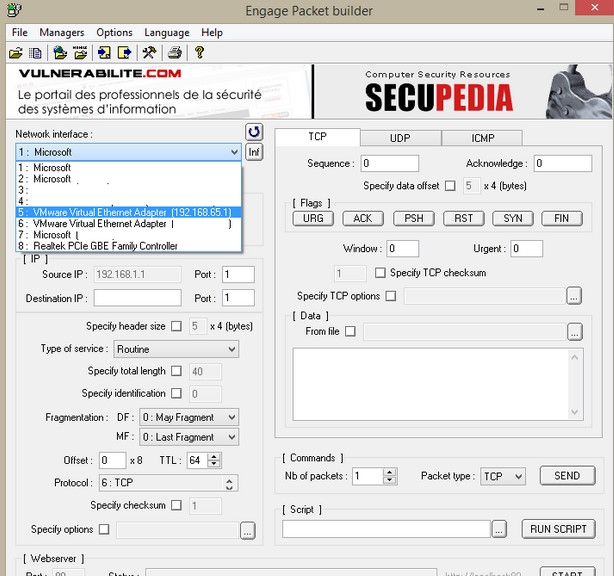
\includegraphics[width=0.5\linewidth]{imgs/engage.jpg}
%  \caption{Screenshot of the Engage Packet Builder tool's interface}
%  \label{fig:engage}
%\end{figure}

\subsection{Aircrack}

Attackers can also utilize Wireshark and a tool called Aircrack-ng in order to crack a WAP’s password. An attacker can sniff out packets with a capable wireless card and capture them utilizing Wireshark. If the attacker is able to capture the correct type of packets, then they can use Aircrack-ng to brute force crack the password. Once the attacker has the encryption password then they can see the data behind all of the packets which could be sensitive data the authorized user of the network does not want to share. 
%Below is a screenshot of an example of Aircrack-ng cracking a password utilizing a brute force method:

\begin{figure}[H]
  \centering
  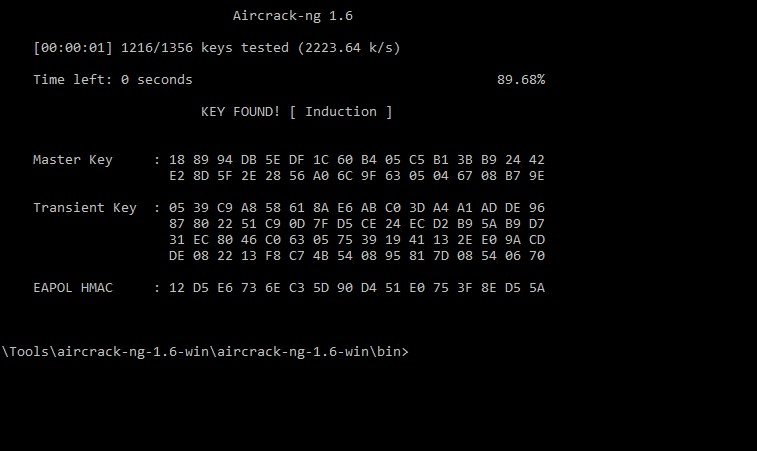
\includegraphics[width=0.5\linewidth]{imgs/aircrack.jpg}
  \caption{Screenshot of the Engage Packet Builder tool's interface}
  \label{fig:aircrack}
\end{figure}

\subsection{Universal Forensic Extraction Device}

The term “mobile devices” encompasses a wide array of gadgets ranging from mobile phones, smartphones, tablets, and GPS units to wearables and PDAs” \cite{Kostadinov_2019}. Similarly to WiFi, mobile devices have become part of the everyday norm for people. A person can usually not go more than 10 minutes without checking their mobile phone unless they are asleep. Mobile devices such as cell phone can contain a ton of personal information, from banking information to passwords and because of that, mobile devices are a key in some investigations and a target for attackers. 
UFED (Universal Forensic Extraction Device) by Cellebrite is a powerful licensed tool for mobile forensics that allows an investigator to bypass pattern, password or PIN locked devices on both Android and iOS devices, collect data from phones, SIM cards, SD cards, GPS devices, and access data from a variety of different apps. 
%Below is a screenshot of one of the UFED menu lists:

%\begin{figure}[H]
%  \centering
%  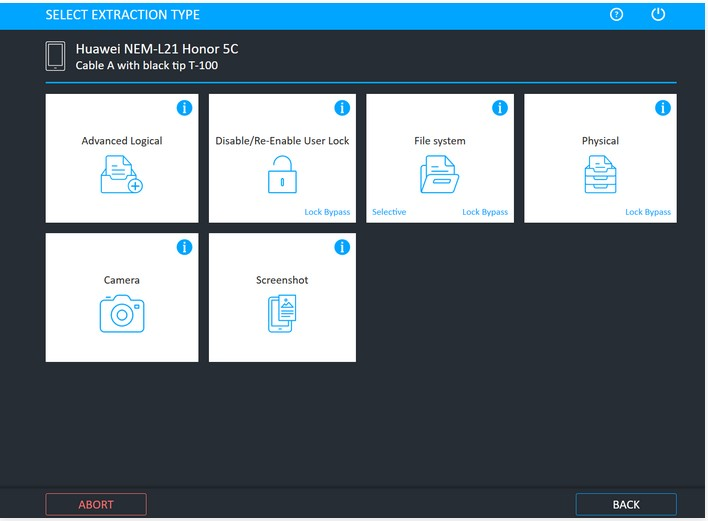
\includegraphics[width=0.5\linewidth]{imgs/ufed.jpg}
%  \caption{Screenshot of the UFED menu lists}
%  \label{fig:ufed}
%\end{figure}

\subsection{iOS Forensic Toolkit}

For iOS specific forensics, the Elcomsoft iOS Forensic Toolkit is extremely useful. This tool can extract all of the data on an iOS device to include, backups, crash logs, media, shared files and can automatically disable screen lock once a device is connected. This tool will work with and iOS device including Apple watches and TV. %Below is a screenshot of the iOS Forensic Toolkit’s main menu:

%\begin{figure}[H]
%  \centering
%  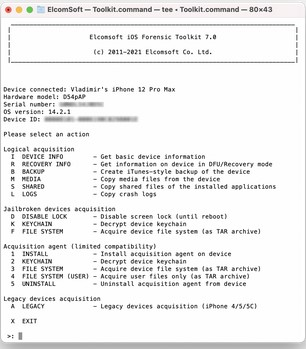
\includegraphics[width=0.5\linewidth]{imgs/ftk.jpg}
%  \caption{Screenshot of iOS Forensic Toolkit’s main menu}
%  \label{fig:ftk}
%\end{figure}

\subsection{Oxygen}

Oxygen Forensic Detective is another powerful tool for mobile forensics. This tool is not only useful for cell phones, but also useful for conducting forensics on IoT devices, device backups, UICC and media cards, drone, and cloud services. It has similar capabilities to the last two mobile forensic tools discussed in that it can bypass screen locks and then extract data. 
%Below is a screenshot of Oxygen Forensic Detective:

\begin{figure}[H]
  \centering
  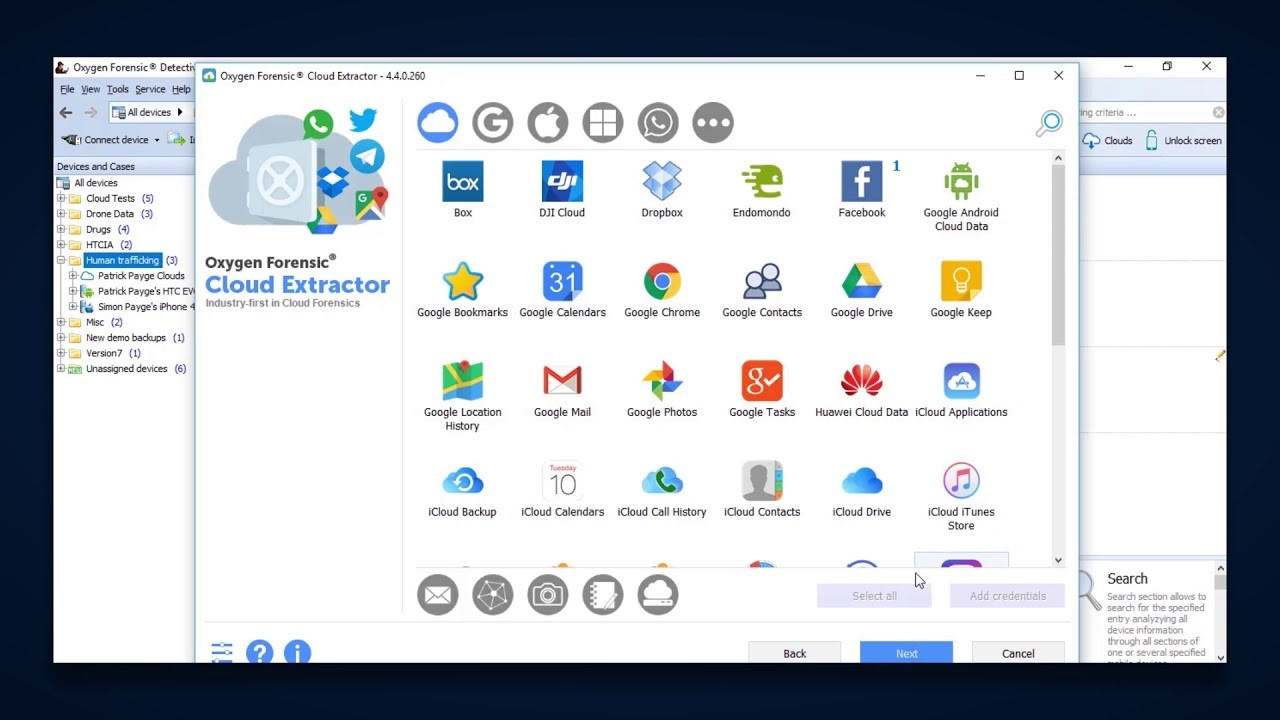
\includegraphics[width=0.5\linewidth]{imgs/oxygen.jpg}
  \caption{Screenshot of Oxygen Forensic Detective}
  \label{fig:oxygen}
\end{figure}
 
Overall, this was just a small sample size of the available tools for that can be used for 802.11 and mobile forensics. There are several different vendors that supply a variety of forensic tools that can be used for law enforcement, government agencies and if in the wrong hands can be used by attackers. As technology becomes more advanced and encryption methods become harder to bypass, tools will continue to have to be upgraded or developed in order to keep up with the ability to conduct successful sound forensic investigations.


\section{Conclusion}

While wireless technology has been around for many decades, it was not until the mid-2000s that it began to take over the world. Nearly every category of electronic devices has a wireless entry. Many of these devices are not manufactured for long term use and wireless security is a mere afterthought. Many IOT devices lack encryption or user authentication protocols. Newer research is finding that these devices may become conduits for bad actors to gain backdoor entries to networks. Luckily, Digital Forensic and Incident Response (DFIR) professionals and researchers are hard at work understanding these technologies to help prevent our wireless infrastructure. As result of their work, new tools have been developed to find malicious artifacts, evidentiary artifacts, and to probe for vulnerabilities. 


\bibliographystyle{style/ACM-Reference-Format}
\bibliography{references}

\end{document}
\endinput
%%
